\documentclass[]{scrreprt}
\usepackage{amsmath,amsfonts,graphicx}

\def\species{\mathrm{sp}}
\def\phase{\mathrm{ph}}
\def\massfrac{\chi}
\def\flux{\mathbf{F}}
\def\darcyvel{\mathbf{v}}
\def\energydens{\mathcal{E}}
\def\d{\mathrm{d}}

\newcommand{\uo}{\mbox{UO\textsubscript{2}}\xspace}

\setcounter{secnumdepth}{3}


\begin{document}


\title{Newton-Cooling Tests}
\author{CSIRO}
\maketitle

\tableofcontents

\chapter{Newton cooling from a bar}


These tests demonstrate that MOOSE behaves correctly when a simulation
contains a sink.  The sink is a piecewise linear function of pressure.

Darcy's equation for (single-phase) flow through a fully saturated medium without
gravity and without sources is
\begin{equation}
\frac{\partial}{\partial t}\phi\rho = \nabla_{i}\left(\frac{\rho
  \kappa_{ij}}{\mu} \nabla_{j}P \right) \ ,
\end{equation}
with the following notation:
\begin{itemize}
\item $\phi$ is the medium's porosity;
\item $\rho$ is the fluid density;
\item $\kappa_{ij}$ is the permeability tensor;
\item $\mu$ is the fluid viscosity;
\item $\partial/\partial t$ and $\nabla_{i}$ denote the time and spatial derivatives, respectively.
\end{itemize}
Using $\rho \propto
\exp(P/B)$, where $B$ is the fluid bulk modulus, Darcy's equation
becomes
\begin{equation}
\frac{\partial}{\partial t}\rho = \nabla_{i}\alpha_{ij}\nabla_{j}\rho \ ,
\end{equation}
with
\begin{equation}
\alpha_{ij} = \frac{\kappa_{ij}B}{\mu\phi} \ .
\end{equation}
Here the porosity and bulk modulus are assumed to be constant in space
and time.

Consider the one-dimensional case where a bar sits between $x=0$ and
$x=L$ with initial pressure distribution so $\rho(x,t=0) = \rho_{0}(x)$.
Maintain the end $x=0$ at constant pressure, so that $\rho(x=0, t) =
\rho_{0}(0)$.  At the end $x=L$, prescribe a sink flux
\begin{equation}
\left.\frac{\partial\rho}{\partial x}\right|_{x=L} = -C\left(\rho -
\rho_{e}\right)_{x=L} \ ,
\end{equation}
where $\rho_{e}$ is a fixed quantity (``e'' stands for ``external''),
and $C$ is a constant conductance.  This corresponds to the flux
\begin{equation}
\left.\frac{\partial P}{\partial x}\right|_{x=L} = -CB\left(1 -
e^{(P_{e}-P)/B}\right)_{x=L} \ ,
\end{equation}
which can easily be coded into a MOOSE input file: the flux is
$\rho\kappa\nabla P/\mu = -CB\kappa(e^{P/B} - e^{P_{e}/B})/\mu$, and
this may be represented by a piecewise linear function of pressure.

The solution of this problem is well known and is
\begin{equation}
\rho(x, t) = \rho_{0}(0) - \frac{\rho_{0}(0) - \rho_{e}}{1 + LC}Cx +
\sum_{n=1}^{\infty} a_{n}\sin \frac{k_{n}x}{L}e^{-k_{n}^{2}\alpha
  t/L^{2}} \ ,
\end{equation}
where $k_{n}$ is the $n^{\mathrm{th}}$ positive root of the equation
$LC\tan k + k=0$  ($k_{n}$ is a little bigger than
$(2n-1)\pi/2$), and $a_{n}$ is determined from
\begin{equation}
a_{n}\int_{0}^{L}\sin^{2}\frac{k_{n}x}{L}\,\mathrm{d}x =
\int_{0}^{L}\left(\rho_{0}(x) - \rho_{0}(0) + \frac{\rho_{0}(0) -
  \rho_{e}}{1 + LC}Cx\right)\sin \frac{k_{n}x}{L}\,\mathrm{d}x \ ,
\end{equation}
which may be solved numerically (Mathematica is used to generate
the solution in Figure~\ref{nc.fig}).

\noindent The problem is solved in MOOSE using the following parameters:
\begin{center}
\begin{tabular}{|ll|}
\hline
Bar length & 100\,m \\
Bar porosity & 0.1 \\
Bar permeability & $10^{-15}$\,m$^{2}$ \\
\hline
Gravity & 0 \\
\hline
Water density & 1000\,kg.m$^{-3}$ \\
Water viscosity & 0.001\,Pa.s \\
Water bulk modulus & 1\,MPa \\
\hline
Initial porepressure $P_{0}$ & 2\,MPa \\
Environmental pressure $P_{e}$ & 0 \\
\hline
Conductance $C$ & 0.05389\,m$^{-1}$ \\
\hline
\end{tabular} \\
\end{center}
This conductance is chosen so at steadystate $\rho(x=L)=2000$\,kg.m$^{-3}$.

The problem is solved using 1000 elements along the $x$ direction
($L=100$\,m), and using 100 time-steps of size $10^6$\,s.  Using fewer
elements or fewer timesteps means the agreement with the theory is
marginally poorer.  Two tests are performed: one with transient flow,
and one using the steadystate solver.  In this case the initial
condition is $P=2-x/L$\,MPa, since the uniform $P=2$\,MPa does not
converge.  The results are shown in Figure~\ref{nc.fig}.

\begin{figure}[htb]
\begin{center}
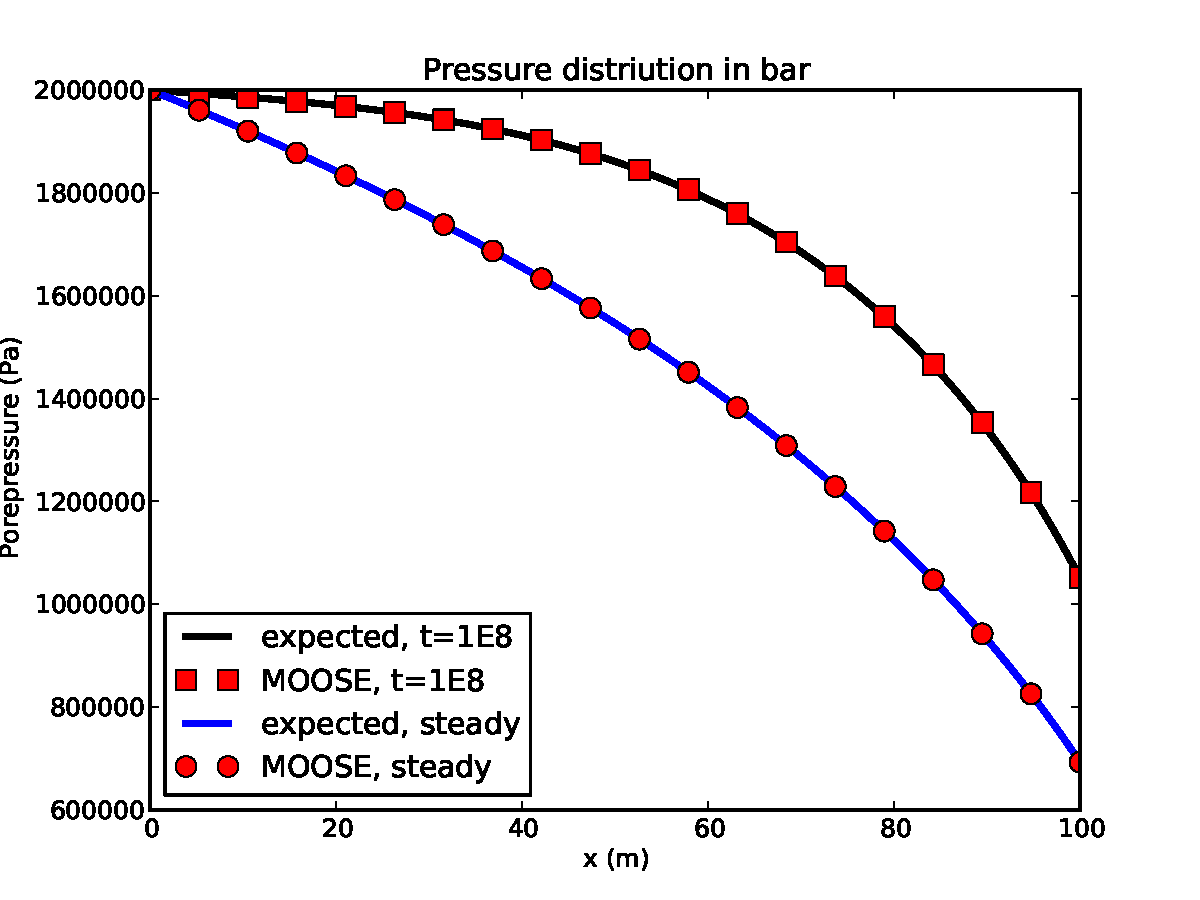
\includegraphics[width=17cm]{nc.pdf}
\caption{The porepressure in the bar at $t=10^{8}$\,s, and at
  steadystate.  The pressure at $x=0$ is held fixed, while the sink is
  applied at $x=100$\,m.  MOOSE agrees well with theory demonstrating
  that piecewise-linear sinks/sources and single-phase Darcy fluid
  flow are correctly implemented in MOOSE.}
\label{nc.fig}
\end{center}
\end{figure}

\end{document}

